\chapter{Experiment and Result}
brief of experiment and result.
\section{Experiment}
Please tell how the experiment conducted from method.

\section{Result}
Please provide the result of experiment

\section{Andri Fajar Sunandhar/1164065}

\subsection{Teori}
\begin{enumerate}
\item Klasifikasi teks
	\par Klasifikasi Teks adalah salah satu tugas penting dan tipikal dalam supervised machine learning (ML). Teks dapat menjadi sumber informasi yang sangat kaya, tetapi mengekstraksi wawasan darinya bisa sulit dan memakan waktu karena sifatnya yang tidak terstruktur.
	\begin{figure}[ht]
		\centering
		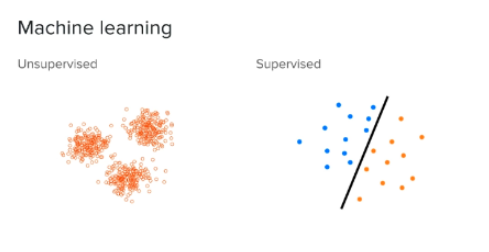
\includegraphics[scale=0.5]{figures/AFS/k1.png}
		\caption{Klasifikasi teks}
		\label{contoh}
	\end{figure}
	
\item Mengapa Klasifikasi Bunga tidak dapat menggunakan machine learning
	\par Dikarenakan tidak semua bunga memliki ciri - ciri yang sama. Atau dalam kata lain terdapat data noise dalam klasifikasi bunga sehingga tidak bisa menggunakan machine learning.
	\begin{figure}[ht]
		\centering
		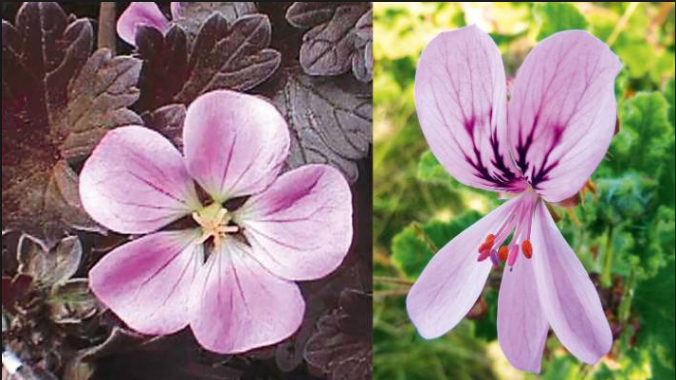
\includegraphics[scale=0.5]{figures/AFS/k2.png}
		\caption{Klasifikasi bunga}
		\label{contoh}
	\end{figure}

\item Teknik pembelajaran mesin pada teks YouTube
	\par Kita ambil sebuah kasus yang semua orang telah ketahui dan juga pahami. Kasus tersebut yaitu perekomendasian video dari pencarian menggunakan "text / kata" di  Youtube. Pada saat menggunakan Youtube terdapat Mchine Learning yang bekerja dan memproses perintah ataupun aktivitas tersebut, dimana akan memfilter secara otomatis video yang disesuaikan dengan "keyword" yang kita masukkan sehingga memberikan keluaran video dengan keyword yang benar. Adapula pada saat kita sedang menonton video di YouTube, pada bagian sebelah kanan ( tampilan Youtube ) terdapat 'Up Next' yang menampilkan beberapa video serupa yang sedang ditonton. Dan ketika mengklik salah satu video dari baris tersebut, maka YouTube akan mengingatnya dan menggunakan kata yang tertera sebagai referensi kembali sehingga akan memberikn kemudahan pada pencarian yang lannya, Dan disitulah mesin belajar sendiri dan menyimpan data secara berkala sehingga berkembang. 

	\begin{figure}[ht]
		\centering
		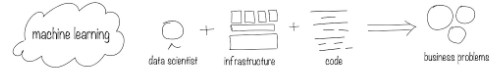
\includegraphics[scale=0.5]{figures/AFS/k3.jpeg}
		\caption{Teknik YouTube}
		\label{contoh}
	\end{figure}

\item Vectorisasi Data
	\begin{itemize}
		\item Pembagian dan pemecahan data, dan kemudian dilakukan perhitungan datanya. Vektorisasi juga dapat dimaksudkan dengan setiap data yang mungkin dipetakan ke integer tertentu. Yang mana data tersebut dalam bentuk data vektor diperoleh dalam bentuk koordinat titik yang menampilkan, menempatkan dan menyimpan data spasial dengan menggunakan titik, garis atau area (poligon). 
	\end{itemize}
	
\item Bag of word
	\par Bag-of-words ialah sebuah gambaran sederhana digunakan dalam pengolahan bahasa alami dan pencarian informasi. Dikenal sebagai model ruang vektor. Pada model ini, tiap kalimat dalam dokumen digambarkan sebagai token, mengabaikan tata bahasa dan bahkan urutan kata namun menghitung frekuensi kejadian atau kemunculan kata dari dokumen.
	\begin{figure}[ht]
		\centering
		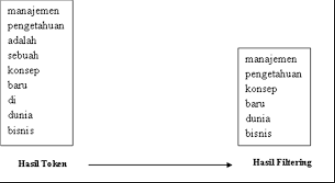
\includegraphics[scale=0.5]{figures/AFS/k4.png}
		\caption{Bag of Word}
		\label{contoh}
	\end{figure}
	
\item TF-IDF
	\par TF-IDF atau TFIDF, adalah kependekan dari istilah frekuensi dokumen terbalik, dimana merupakan statistik numerik yang dimaksudkan untuk mencerminkan betapa pentingnya sebuah kata untuk sebuah dokumen dalam kumpulan atau kumpulan. Nilai tf-idf meningkat secara proporsional dengan berapa kali sebuah kata muncul dalam dokumen dan diimbangi dengan jumlah dokumen dalam korpus yang mengandung kata, yang membantu menyesuaikan fakta bahwa beberapa kata muncul lebih sering secara umum.
	\begin{figure}[ht]
		\centering
		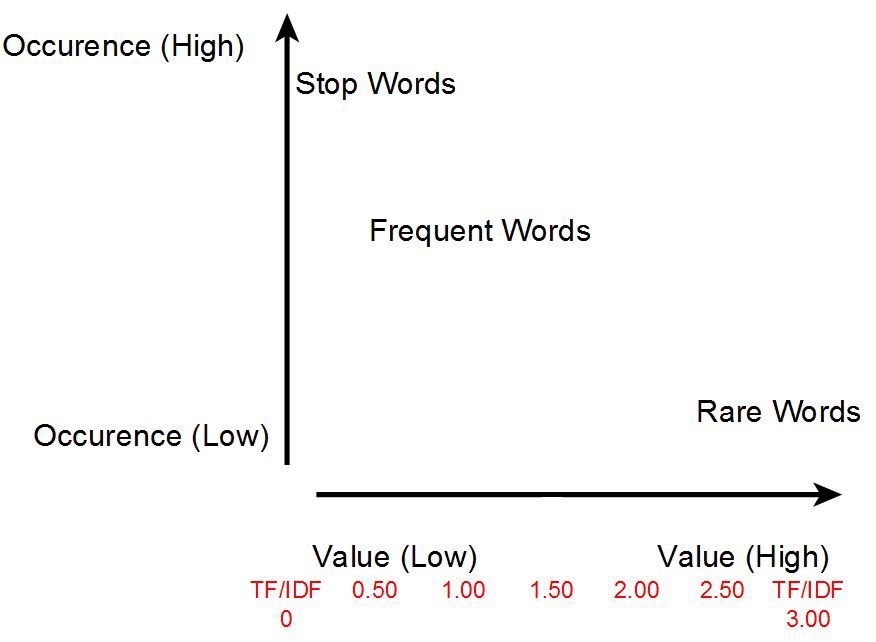
\includegraphics[scale=0.5]{figures/AFS/k5.jpeg}
		\caption{TF IDF}
		\label{contoh}
	\end{figure}
\end{enumerate}


\subsection{Praktek Program}
\begin{enumerate}
\item Aplikasi sederhana menggunakan pandas
	\par Berikut adalah contoh aplikasi sederhana yang dibuat menggunakan pandas :
	
		\begin{figure}[ht]
		\centering
		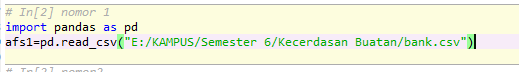
\includegraphics[scale=0.5]{figures/AFS/a1.png}
		\caption{Pandas}
		\label{contoh}
		\end{figure}
		
	\begin{enumerate}
	\item 1 = memanggil library pandas sebagai pd
	\item 2 = membuat varible afs1 untuk membaca file .csv (bank.csv)
	\end{enumerate}
	
	\par Hasil dari pandas menampilkan data dari bank.csv :
	
		\begin{figure}[ht]
		\centering
		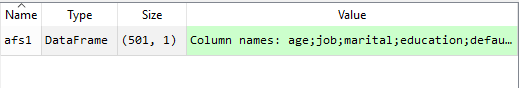
\includegraphics[scale=0.5]{figures/AFS/a2.png}
		\caption{Hasil Pandas}
		\label{contoh}
		\end{figure}	
	
\item Memecah dataframe menjadi 2 dataframe
	\par Memecah dataframe :
	
		\begin{figure}[ht]
		\centering
		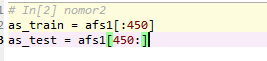
\includegraphics[scale=0.5]{figures/AFS/a3.png}
		\caption{Memecah dataframe}
		\label{contoh}
		\end{figure}
	
	\begin{enumerate}
	\item 1 = Melakukan split data training sebanyak 450
	\item 2 = dan sisanya sebagai data testing
	\end{enumerate}
	
	\par Berikut hasil memecah dataframe menjadi 2 :
	
		\begin{figure}[ht]
		\centering
		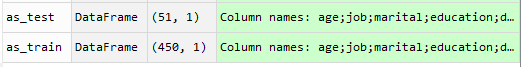
\includegraphics[scale=0.5]{figures/AFS/a4.png}
		\caption{Hasil memecah dataframe}
		\label{contoh}
		\end{figure}
		
\item Vektorisasi dan klasifikasi Decission Tree dari data Youtube03-LMFAO.csv
	
	\par Berikut adalah vektorisasi dan klasifikasi dari data Youtube03-LMFAO.csv
		\begin{figure}[ht]
		\centering
		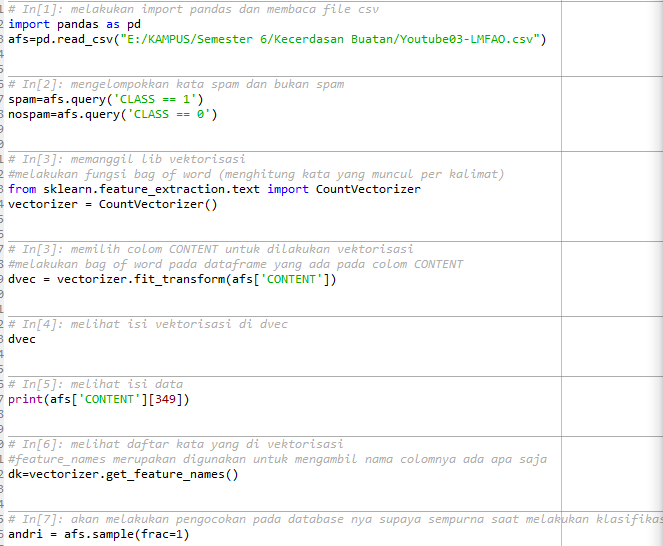
\includegraphics[scale=0.5]{figures/AFS/a5.png}
		\caption{Vektorisasi dan klasifikasi}
		\label{contoh}
		\end{figure}
	\begin{enumerate}
	\item 1 = Melakukan import pandas dan membaca file Youtube03-LMFAO.csv
	\item 2 = Mengelompokan data spam bukan spam
	\item 3 = Memanggil library vektorisasi dan menghitung kata yang muncul per kalimat
	\item 4 = Memilih kolom CONTENT untuk melakukan vektorisasi
	\item 5 = Melihat isi vektorisasi
	\item 6 = Melihat isi data pada kolom CONTENT namun pada bagian kolom ke 349
	\item 7 = Melihat daftar kata yang di vektorisasi
	\item 8 = Akan melakukan pengocokan pada data nya supaya hasilnya sempurna ketika melakukan klasifikasi
	\end{enumerate}
	
	\par Berikut adalah Decission Tree Youtube03-LMFAO.csv
		\begin{figure}[ht]
		\centering
		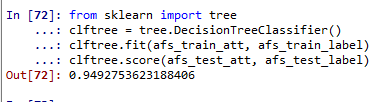
\includegraphics[scale=0.5]{figures/AFS/a6.png}
		\caption{Decission Tree}
		\label{contoh}
		\end{figure}
	\par Dalam gambar Decission Tree dijelaskan bahwa library tree dari sklearn. Dan mendifinisikan variable untuk memanggil Decission Tree Classifisier yang kemudian dilakukan fit atau pengujian terhadap data training.dan untuk menghitung score dari data testing. Yang menghasilkan outputan sebanyak 0.9492753623188406 .
	

\item Klasifikasikan dari data vektorisasi dengan klasifikasi SVM
	\par Berikut adalah klasifikasikan dari data vektorisasi dengan klasifikasi SVM
		\begin{figure}[ht]
		\centering
		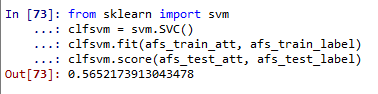
\includegraphics[scale=0.5]{figures/AFS/a7.png}
		\caption{Hasil klasifikasi SVM}
		\label{contoh}
		\end{figure}
	\par Dalam gambar SVM dijelaskan bahwa svm mengimport library dari sklearn kemudian membuat variable clfsvm, fit tersebut membaca data training atribute dan data training label, score membaca data testing attribute dan data testing label sehingga menghasilkan outputan 0.5652173913043478
	
\item Klasifikasikan dari data vektorisasi dengan klasifikasi Decission Tree
	\par Maksud dari gambar vektorisasi adalah hasil dari impor dataset
	\par Berikut adalah Decission Tree
		\begin{figure}[ht]
		\centering
		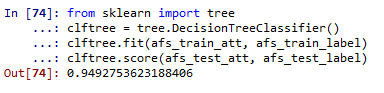
\includegraphics[scale=0.5]{figures/AFS/a8.png}
		\caption{Decission Tree}
		\label{contoh}
		\end{figure}
	\par Dalam gambar Decission Tree dijelaskan bahwa library tree dari sklearn. Dan mendifinisikan variable untuk memanggil Decission Tree Classifisier yang kemudian dilakukan fit atau pengujian terhadap data training.dan untuk menghitung score dari data testing. Yang menghasilkan outputan sebanyak 0.9492753623188406 .

\item Plot confusion matrix menggunakan matplotlib
	\par hasil dari ploting confusion matrix :
		\begin{figure}[ht]
		\centering
		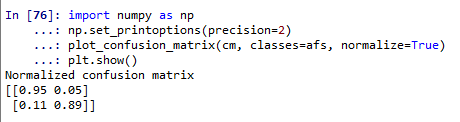
\includegraphics[scale=0.5]{figures/AFS/a9.png}
		\caption{ploting confusion matrix}
		\label{contoh}
		\end{figure}
	\par Dari gambar dijelaskan menginport library numpy sebagai np, kemudian menampilkan precision 2 dan melakukan plot confusion matrix dari classes afs dan kemudian akan melakukan normalisasi. sehingga hasil normalisasi seperti pada gambar tersebut.

\item Program cross validation
	\par Berikut adalah hasil dari program cross validation
		\begin{figure}[ht]
		\centering
		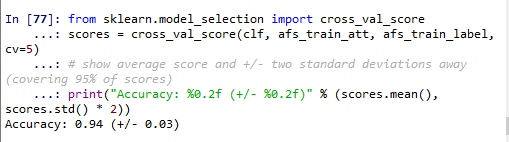
\includegraphics[scale=0.5]{figures/AFS/a10.png}
		\caption{Program cross validation}
		\label{contoh}
		\end{figure}
		
	\par Daru gambar tersebut dijelaskan cara menghitung scores dari cross validation data training attribute dan data training label kemudian dikali 2 sehingga menghasilkan akurasi 0.94.
	
\item Program pengamatan komponen informasi
	\par  Hasil dari program pengamatan komponen informasi
		\begin{figure}[ht]
		\centering
		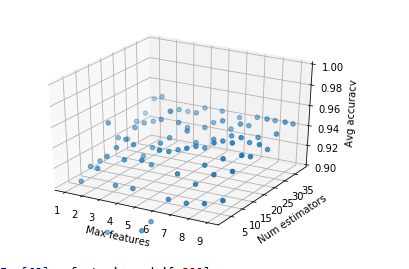
\includegraphics[scale=0.5]{figures/AFS/n11.png}
		\caption{Program pengamatan komponen informasi}
		\label{contoh}
		\end{figure}
		
	\par Gambar tersebut adalah diagram informasi dari dataset yang digunakan.

\end{enumerate}

\subsection{Penanganan Error}
\begin{enumerate}
	\item skrinsut error
		\begin{figure}[ht]
		\centering
		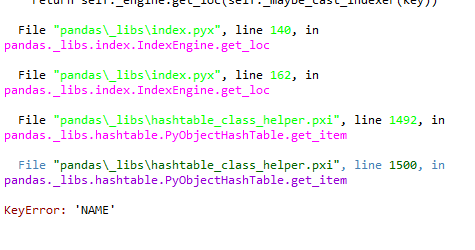
\includegraphics[scale=0.5]{figures/AFS/a12.png}
		\caption{skrinsut error}
		\label{contoh}
		\end{figure}
	\item Tuliskan kode eror dan jenis errornya
		\begin{itemize}
		\item Kode error = KeyError: 'NAME'
		\item Jenis error = KeyError
		\end{itemize}
	\item Solusi pemecahan masalah error
		\par Solusinya adalah mengganti nama field NAME dengan CONTENT, dikarenakan didalam data tersebut tidak ada field NAME. Kemudian akan menampilkan data CONTENT hanya pada baris ke 349. 
		\begin{figure}[ht]
		\centering
		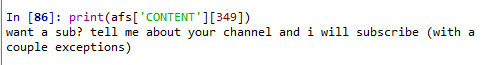
\includegraphics[scale=0.5]{figures/AFS/a13.png}
		\caption{Solusi error}
		\label{contoh}
		\end{figure}
	
\end{enumerate}